\section{Cryptographic security definitions}
\label{sec:ac}

\subsection{Real-world ideal-world paradigm}
\label{sec:ac.realideal}

Cryptographic schemes are not usually perfectly secure. Rather, they provide a certain level of security that is quantified by one or several parameters. Take for instance an encryption scheme. It could only be called perfectly secure if we had a guarantee that an adversary can learn absolutely nothing about the encrypted message \--- something that turns out to be impossible to achieve in practice. Still, we have encryption schemes, e.g., those built in quantum cryptography, that are ``almost perfectly secure''. So we need a quantitative definition that makes precise what this means.

Devising sensible quantitative definitions can be challenging.  Consider, for instance, a protocol that encrypts quantum information contained in a $d$-dimensional register~$A$ by applying a unitary $U_k$ that depends on a uniformly chosen key $k \in \cK$. It has been proposed, e.g., in \textcite{AS04,HLSW04,DN06}, that the security of such a scheme may be defined by requiring that, for any state $\rho_A$,
\begin{equation} \label{eq:encryption.naive}
  \frac{1}{2}\trnorm{\frac{1}{|\cK|} \sum_{k \in \cK} U_k \rho_A \hconj{U}_k -
    \tau_A} \leq \eps,
\end{equation}
where $\eps \geq 0$ is the security paramter, $\tau_A = \frac{1}{d} I$ is the fully mixed state, and $\trnorm{\cdot}$ denotes the trace norm or
Schatten $1$-norm. The definition has been justified by the argument that an adversary who does not know the key~$k$ cannot distinguish the encryption of the state from $\tau_A$
(except with advantage\footnote{See the text around~\eqref{eq:adv1} for a definition of the notion of a \emph{distinguishing advantage}.} $\eps$). However, it has later been realized that this does not hide
the information in the $A$ system from an adversary who may hold a purification
$R$ of the information~$A$ \cite{ABW09}. To take this into account, one should instead require that,
for any $\rho_{AR}$,
\begin{equation*} %\label{eq:encryption.purification}
  \frac{1}{2}\trnorm{\frac{1}{|\cK|} \sum_{k \in \cK} \left(U_k \otimes I_R
    \right) \rho_{AR} \left(\hconj{U}_k \otimes I_R\right) - \tau_A
    \otimes \rho_R} \leq \eps,
\end{equation*}
where $\rho_R$ is the reduced density operator of $\rho_{AR}$. Note
that, crucially, this criterion is not implied
by~\eqnref{eq:encryption.naive} above \cite{Wat18}.

As another example, early works on Quantum Key Distribution (QKD),
e.g., \textcite{May96,BBBMR00,SP00}, measured the secrecy of a secret
key in terms of the \emph{accessible information}\footnote{This
  captures the information a player may obtain by measuring her
  quantum state, and is formally defined in \eqnref{eq:localqkd} in
  \secref{sec:qkd.other.ai}, see also \textcite{nielsen2010quantum}.}
between the key and all information that may be accessible to an
adversary. In security proofs it was then shown that this value is
small, apparently implying that the key is almost perfectly
secret. Later one has realised, however, that the accessible
information is not a good measure for secrecy: even if this measure is
exponentially small in the key size, an adversary may for example be
able to infer the second part of the key upon seeing the first
part~\cite{KRBM07}. This makes the key unusable for many applications,
such as encryption, as described in detail in
\secref{sec:qkd.other.ai}.

Problems analogous to the ones outlined above are well known in classical cryptography. They were addressed independently by
\textcite{PW00,PW01} and \textcite{Can01}, building on a series of
earlier works~\cite{GMW86,Bea92,MR92,Can00}, with a security paradigm
that we will refer to as the ``real\-/world ideal\-/world'' paradigm.
Its gist lies in quantifying how well some \emph{real} protocol for a
cryptographic task can be distinguished from some \emph{ideal} system
that fulfils the task perfectly.

As a simple (non-cryptographic) example, we consider channel coding, i.e., the task of constructing a noiseless channel form a noisy one. Suppose that Alice
and Bob only have access to a noisy channel, drawn in
\figref{fig:security.channel.noisy}. In order to send a 
message, Alice will encode it in a larger message space that has
redundancies. Upon reception, Bob will decode it, using the redundancies to correct errors~\cite{nielsen2010quantum}. Putting together the encoder, the noisy channel, and the 
decoder, as illustrated in
\figref{fig:security.channel.construction}, gives a new channel. Ideally, this constructed channel, which we call the \emph{real world}, should behave like a perfect, noiseless channel,
\figref{fig:security.channel.noiseless}, which we therefore call the \emph{ideal world}. To quantify how well we achieved this goal, we measure how close the real world is to the ideal world.

\begin{figure}[tb]
  \centering
  \subfloat[Noiseless channel][\label{fig:security.channel.noiseless}A
  noiseless channel that perfectly delivers the message from Alice to
  Bob.]{
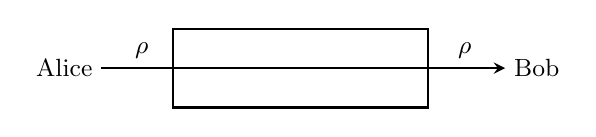
\begin{tikzpicture}[
sArrow/.style={->,>=stealth,thick},
thinResource/.style={draw,thick,minimum width=1.618*2cm,minimum height=1cm}]

\small

\node[thinResource] (channel) at (0,0) {};
\node (alice) at (-3,0) {Alice};
\node (bob) at (3,0) {Bob};

\draw[sArrow] (alice) to node[pos=.1,auto] {$\rho$} node[pos=.9,auto] {$\rho$}  (bob);

\end{tikzpicture}
}

\vspace{6pt}

\subfloat[Noisy channel][\label{fig:security.channel.noisy}A noisy
channel that alters the message sent from Alice to Bob.]{
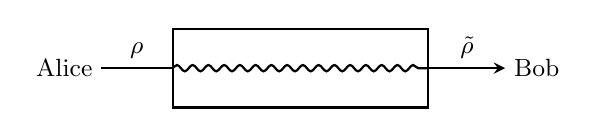
\begin{tikzpicture}[
sLine/.style={-,thick},
nLine/.style={-,thick,decorate,decoration={snake,amplitude=.4mm,segment length=2mm,post length=1mm}},
sArrow/.style={->,>=stealth,thick},
thinResource/.style={draw,thick,minimum width=1.618*2cm,minimum height=1cm}]

\small

\node[thinResource] (channel) at (0,0) {};
\node (alice) at (-3,0) {Alice};
\node (bob) at (3,0) {Bob};

\draw[sLine] (alice) to node[pos=.5,auto] {$\rho$} (channel.west);
\draw[nLine] (channel.west) to (channel.east);
\draw[sArrow] (channel.east) to node[pos=.5,auto] {$\tilde{\rho}$} (bob);

\end{tikzpicture}
}

\vspace{6pt}

\subfloat[Noiseless channel
construction][\label{fig:security.channel.construction}Alice encodes
  her message into a larger space, and Bob decodes upon reception.]{
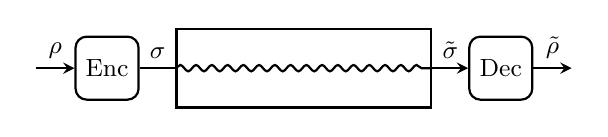
\begin{tikzpicture}[
sLine/.style={-,thick},
nLine/.style={-,thick,decorate,decoration={snake,amplitude=.4mm,segment length=2mm,post length=1mm}},
sArrow/.style={->,>=stealth,thick},
thinResource/.style={draw,thick,minimum width=1.618*2cm,minimum height=1cm},
converter/.style={draw,thick,rounded corners,minimum width=.8cm,minimum height=.8cm}]

\small

\node[thinResource] (channel) at (0,0) {};
\node[converter] (A) at (-2.5,0) {Enc};
\node[converter] (B) at (2.5,0) {Dec};
\node (alice) at (-3.4,0) {};
\node (bob) at (3.4,0) {};

\draw[sArrow] (alice.center) to node[pos=.5,auto] {$\rho$} (A);
\draw[sLine] (A) to node[pos=.5,auto] {$\sigma$} (channel.west);
\draw[nLine] (channel.west) to (channel.east);
\draw[sArrow] (channel.east) to node[pos=.5,auto] {$\tilde{\sigma}$} (B);
\draw[sArrow] (B) to node[pos=.5,auto] {$\tilde{\rho}$} (bob.center);

\end{tikzpicture}
}
\caption[Channels for error
correcting]{\label{fig:security.channels}In these diagrams each box
  represents a reactive system which produces an output upon receiving
  an input. Boxes with rounded corners are local operations performed
  by a party [e.g., encoding and decoding in
  \subref{fig:security.channel.construction}]. The rectangular box is
  a (possibly noisy) channel form Alice to Bob, which upon receiving
  Alice's input produces an output at Bob's end of the channel. The
  arrows represent quantum states being transmitted from one system to
  another.}
\end{figure}

For this, we consider a hypothetical game in which a
\emph{distinguisher} has \emph{black box access} to an unknown system
as shown in \figref{fig:distinguisher}. The unknown system is,
depending on a random bit~$B$, either the real world ($B=0$) or the
ideal world ($B=1$). The term \emph{black box access} means that the
distinguisher is not provided with a description of the system, and in
particular has no direct access to the bit~$B$, but otherwise can
interact arbitrarily with it. In the case of our noiseless channel
construction problem, the distinguisher can generate any joint state
$\rho_{AR}$ it desires, input the $A$ part into the channel, and then
measure the joint state of the channel output and its purification
$R$.  The distinguisher is then asked to guess whether it interacts
with the real world ($B=0$) or with the ideal one ($B=1$). Let $D$ be
a random variable denoting the distinguisher's guess. The
\emph{distinguishing advantage} of the distinguisher is then defined as the
difference between the probabilities that it guesses correctly and
erroneously, namely
\begin{equation} \label{eq:adv1} \left|\Pr[D = 0|B=0] - \Pr[D = 0|B=1]
  \right|.\end{equation} The distinguishing advantage for a class of
distinguishers (e.g., computationally bounded or unbounded
distinguishers), is then defined as the supremum of \eqnref{eq:adv1}
over all distinguishers in this set. For example, in the case of channel coding, the distinguishing advantage for unbounded
distinguishers corresponds to the diamond\-/norm between the
channels~\cite{Wat18}. A protocol is considered secure if the
distinguishing advantage is small \--- or, more accurately, the (level
of) security of a protocol is parametrized by this advantage and the
corresponding class of distinguishers.

\begin{figure}[tb]
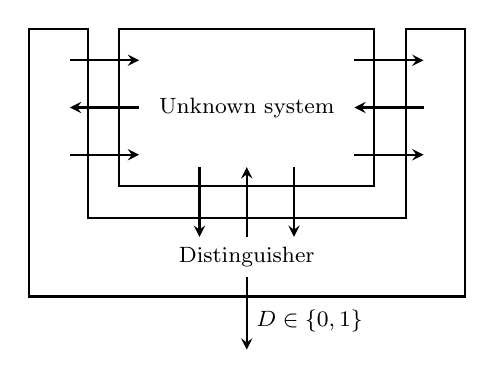
\begin{tikzpicture}[
sArrow/.style={->,>=stealth,thick},
largeResource/.style={draw,thick,minimum width=1.618*2cm,minimum height=2cm},
lrnode/.style={minimum width=1.36*2cm,minimum height=.2cm},
llrnode/.style={minimum width=.2cm,minimum height=1.5cm},
tlrnode/.style={minimum width=.2cm,minimum height=.5cm}]


\small

\def\v{.6}
\def\u{2.27} %1.618+.4+2.5
\def\w{-1.9} %1+.4+.5
%\def\b{10cm}

\node[lrnode] (r1) at (0,\v) {};
\node[lrnode] (r2) at (0,0) {};
\node[lrnode] (r3) at (0,-\v) {};
\node[llrnode] (rr1) at (-\v,0) {};
\node[llrnode] (rr2) at (0,0) {};
\node[llrnode] (rr3) at (\v,0) {};
\node[largeResource] (R) at (0,0) {\footnotesize Unknown system};

\draw[thick] (-1.618-1.15,1) -- ++(.75,0) -- ++(0,-2.4)  --
++(1.618*2+.8,0)  -- ++(0,2.4) -- ++(.75,0) -- ++(0,-3.4) --
++(-1.618*2-2.3,0) -- cycle;

\node at (0,\w) {\footnotesize Distinguisher};
\node[tlrnode] (dd1) at (-\v,\w) {}; 
\node[tlrnode] (dd2) at (0,\w) {}; 
\node[tlrnode] (dd3) at (\v,\w) {};
\node[inner sep=0] (d1) at (-\u,\v) {};
\node[inner sep=0] (d2) at (-\u,0) {};
\node[inner sep=0] (d3) at (-\u,-\v) {};
\node[inner sep=0] (d4) at (\u,\v) {};
\node[inner sep=0] (d5) at (\u,0) {};
\node[inner sep=0] (d6) at (\u,-\v) {};
\node[inner sep=0] (d0) at (0,\w-.5-.7) {};

\draw[sArrow] (rr1) to (dd1);
\draw[sArrow] (dd2) to (rr2);
\draw[sArrow] (rr3) to (dd3);
\draw[sArrow] (d1) to (r1);
\draw[sArrow] (r2) to (d2);
\draw[sArrow] (d3) to (r3);
\draw[sArrow] (r1) to (d4);
\draw[sArrow] (d5) to (r2);
\draw[sArrow] (r3) to (d6);
\draw[sArrow] (dd2) to node[auto,pos=.6] {\footnotesize $D \in \{0,1\}$} (d0);

%%%%%%%%%%%%

% \node[xshift=\b,lrnode] (i1) at (0,\v) {};
% \node[xshift=\b,lrnode] (i2) at (0,0) {};
% \node[xshift=\b,lrnode] (i3) at (0,-\v) {};
% \node[xshift=\b,llrnode] (ii1) at (-\v,0) {};
% \node[xshift=\b,llrnode] (ii2) at (0,0) {};
% \node[xshift=\b,llrnode] (ii3) at (\v,0) {};
% \node[xshift=\b,largeResource] (I) at (0,0) {\footnotesize Ideal system};


% \draw[xshift=\b,thick] (-1.618-1.15,1) -- ++(.75,0) -- ++(0,-2.4)  --
% ++(1.618*2+.8,0)  -- ++(0,2.4) -- ++(.75,0) -- ++(0,-3.4) --
% ++(-1.618*2-2.3,0) -- cycle;

% \node[xshift=\b] at (0,\w) {\footnotesize Distinguisher};
% \node[xshift=\b,tlrnode] (ee1) at (-\v,\w) {}; 
% \node[xshift=\b,tlrnode] (ee2) at (0,\w) {}; 
% \node[xshift=\b,tlrnode] (ee3) at (\v,\w) {};
% \node[xshift=\b,inner sep=0] (e1) at (-\u,\v) {};
% \node[xshift=\b,inner sep=0] (e2) at (-\u,0) {};
% \node[xshift=\b,inner sep=0] (e3) at (-\u,-\v) {};
% \node[xshift=\b,inner sep=0] (e4) at (\u,\v) {};
% \node[xshift=\b,inner sep=0] (e5) at (\u,0) {};
% \node[xshift=\b,inner sep=0] (e6) at (\u,-\v) {};
% \node[xshift=\b,inner sep=0] (e0) at (0,\w-.5-.7) {};

% \draw[sArrow] (ii1) to (ee1);
% \draw[sArrow] (ee2) to (ii2);
% \draw[sArrow] (ii3) to (ee3);
% \draw[sArrow] (e1) to (i1);
% \draw[sArrow] (i2) to (e2);
% \draw[sArrow] (e3) to (i3);
% \draw[sArrow] (i1) to (e4);
% \draw[sArrow] (e5) to (i2);
% \draw[sArrow] (i3) to (e6);
% \draw[sArrow] (ee2) to node[auto,pos=.6] {\footnotesize $0,1$} (e0);

\end{tikzpicture}


\caption[Distinguishing systems]{\label{fig:distinguisher}In the real-world ideal-world paradigm, security is defined in terms of indistinguishability. A distinguisher  has black-box access to a system that, depending on an unknown bit $B$, is either the real cryptographic protocol ($B=0$) or an ideal functionality ($B=1$). After interacting with
  the system, the distinguisher outputs a guess $D$ for $B$. The real protocol is considered as secure as the ideal system if the success probability $\Pr[D=B]$ of the best possible distinguisher is close to that of a random guess, i.e., to~$\frac{1}{2}$.}
\end{figure}

In its essence, the real-world ideal-world paradigm avoids defining
\emph{security}; instead, it provides a simple description, the ideal
world, of what should happen in the real world. In the example of
channel coding, the real world might involve a complex noise model as
well as encoding and decoding operations, whereas the ideal world is
just an identity map.  When evaluating whether such a security
statement is appropriate, one asks whether the ideal world captures
what we need, or whether one should design a different ideal world.

A crucial property of the real-world ideal-world paradigm is that the resulting notion of security is \emph{composable}.  This means that the security of a protocol is guaranteed even if it is composed with other protocols to form a larger cryptographic system. In fact, to ensure composability,  the notion of distinguishability has to be chosen appropriately. Specifically, the distinguisher must have access jointly to
all information available normally to the honest parties as well as to the adversary. The role of the distinguisher is hence to capture ``the rest of the world'', everything that exists around the system of interest. In particular, the distinguisher may choose the inputs to the protocol (that might come from a previously run protocol), receive its outputs (that could be used in a subsequent protocol), and  simultaneously take the role of the adversary, possibly eavesdropping on the communication channels and tampering with messages. 

% The ``real-world ideal-world'' paradigm is the basis of modern security definitions in quantum cryptography.  While the details of this definition for the case of QKD will be treated in \secref{sec:qkd}, it is already here possible to understand the intuition behind it. If the distinguisher is connected to the real QKD protocol ($B=0$), it has access to the key~$K$ generated by the protocol as well as to all information~$E$ that would be accessible to an eavesdropper. This is then compared to a situation where the distinguisher is connected to an ideal system ($B=1$), which generates a perfectly uniform key~$K$ that is completely independent from~$E$. If the distinguishing advantage is small, this means that the real QKD protocol shows essentially the same behaviour as the ideal system, independently of the behaviour of the world around it, which is instantiated by the distinguisher. The protocol can thus be considered \emph{secure}.


\subsection{The Abstract Cryptography framework}
\label{sec:ac.ac}

In modern cryptography, security claims (and their proofs) are usually
phrased within a theoretical framework. The framework does not only
provide a common language, but also ensures composability, in the
sense described above. That is, security claims that hold for
individual components can be turned into a security claim for a more
complex cryptographic scheme built from them. The first frameworks to
achieve this for classical cryptography are the \emph{reactive
  simulatability framework} of~\textcite{PW00,PW01} and the
\emph{universal composability framework} of~\textcite{Can01}, which
both use the real-world ideal-world paradigm.

These frameworks have been further developed \cite{BPW04,BPW07,CDPW07,Can20} and several variations have been
proposed~\cite{MMS03,MRST06,CCKLLPS06a,CCKLLPS06b,Kus06,HS13}. The differences between them concern mostly how they describe information-processing systems, i.e., how the individual devices carry out computations and how they schedule messages when communicating (e.g., synchronously or asynchronously).  While this modelling was mostly based on classical notions of computation and communication, the frameworks have also been adapted to quantum cryptography by
\textcite{BM04} and \textcite{Unr04,Unr10}. 

In \textcite{MR11} [see also, \textcite{Mau12,MR16}] a framework was
proposed, \emph{Abstract Cryptography} (AC), that is largely
independent of the underlying modelling of the information-processing
devices, and therefore applies equally to classical and quantum
settings. We use it for the presentation here, for it enables a
self-contained description without the need to specify (unnecessary)
technical details.\footnote{The security of QKD could be equivalently
  modelled based on the work of \textcite{Unr10} with minor
  adaptations to capture finite statements instead of only
  asymptotics.}
% Furthermore, the AC framework is strictly more powerful, since
% it allows messages to be sent to a superposition of different players;
% it even allows superpositions of different numbers of messages to be
% generated in superpositions of different orders~\cite{PMMRT17} \---
% though these features are not needed in the current work.
In the following, we briefly describe the two basic paradigms on which
the framework is based, \emph{abstraction} and
\emph{constructibility}.

\paragraph{Abstraction.}
The traditional approach to defining security \--- used in all the
frameworks cited except for AC \--- can be seen as \emph{bottom\-/up}. One
first defines (at a low level) a computational model (e.g., a Turing
machine), and then proceeds by modelling how the machines communicate (e.g., by
writing to and reading from shared tapes). Next, one introduces higher-level notions such as indistinguishability. Finally, these notions are used to define security. 

In contrast, AC uses a \emph{top\-/down} approach. In order to state definitions and develop a theory, one starts from the other end, the highest possible level of abstraction. There, cryptographic systems are simply regarded as elements of a set, which can be combined to form new systems. One then proceeds down to lower levels of abstraction, introducing in each of them the minimum necessary specializations. Only on these lower levels it is modelled how exactly the cryptographic systems process information and how they communicate when they are combined (e.g., synchronously or asynchronously). The notion of indistinguishability is first defined on the highest abstraction level as an (arbitrary) metric on the set of cryptographic systems. On lower abstraction levels it can then be instantiated in different ways, e.g., to capture the distinguishing power of a computationally bounded or unbounded environment. 

Abstraction has not only the advantage that it generalises the treatment, but it usually also simplifies it, as unnecessary specificities are avoided.  It may be compared, for instance, to the use of group theory in mathematics, which is an abstraction of more special concepts such as matrix multiplication.  In a bottom\-/up approach, one would
start introducing a rule for taking the product between matrices and then, based on that rule, study the properties of the multiplication operation. In contrast to this, the
top\-/down approach taken here corresponds to first defining the (abstract) multiplication group and prove theorems already on this level. 

%Matrix multiplication could then be introduced later as a special case.

 % It is important to point out that theorems proven at a
% certain (high) level of abstraction are completely precise (as they
% are mathematical theorems). This is true without instantiations of the
% lower levels, which is exactly the point of abstraction.


\paragraph{Constructibility.}
Cryptography can be regarded as a resource theory, where certain
desired resources are \emph{constructed} from a set of given
resources.\footnoteremember{fn:resourcetheory}{This view is widespread
  in cryptography and made formal by composable frameworks \--- e.g.,
  \textcite{PW00,PW01,Can01,MR11}. Resource theories have also been
  used in many different ways to capture (certain aspects of) quantum
  mechanics, see the recent reviews \textcite{SAP17,CG19}.} The
constructions are defined by protocols. For example, a QKD protocol
uses a quantum communication channel together with an authentic
channel\footnote{An authentic channel guarantees that the message
  received comes from the legitimate sender, and has not been tampered
  with or generated by an adversary.} as resources to construct the
resource of a secret key. This latter resource may then be used by
other protocols, e.g., an encryption protocol, to construct a secure
communication channel, which is again a resource. Similarly, the
authentic channel used by the QKD protocol can itself be constructed
from an insecure channel resource and short (uniform) secret key
\cite{WC81}. And given a weak secret key (i.e., not necessarily
uniform and not perfectly correlated randomness shared by the
communication partners) and 2-way insecure channels, one may construct
an almost perfect secret key (i.e., uniform and perfectly correlated
randomness) using so-called non\-/malleable
extractors~\cite{RW03,DW09,ACLV19}. Composing the authentication
protocol with the QKD protocol results in a scheme which constructs a
long secret key from a short secret key and insecure channels \--- and
composing this again with non\-/malleable extractors constructs this
long key from only a weak key and insecure channels. Part of the
resulting long secret key can be used in further rounds of
authentication and QKD to produce even more secret key. This is
illustrated in \figref{fig:construction}, and discussed in detail in
\secref{sec:smt}.

\begin{figure*}[tbp]

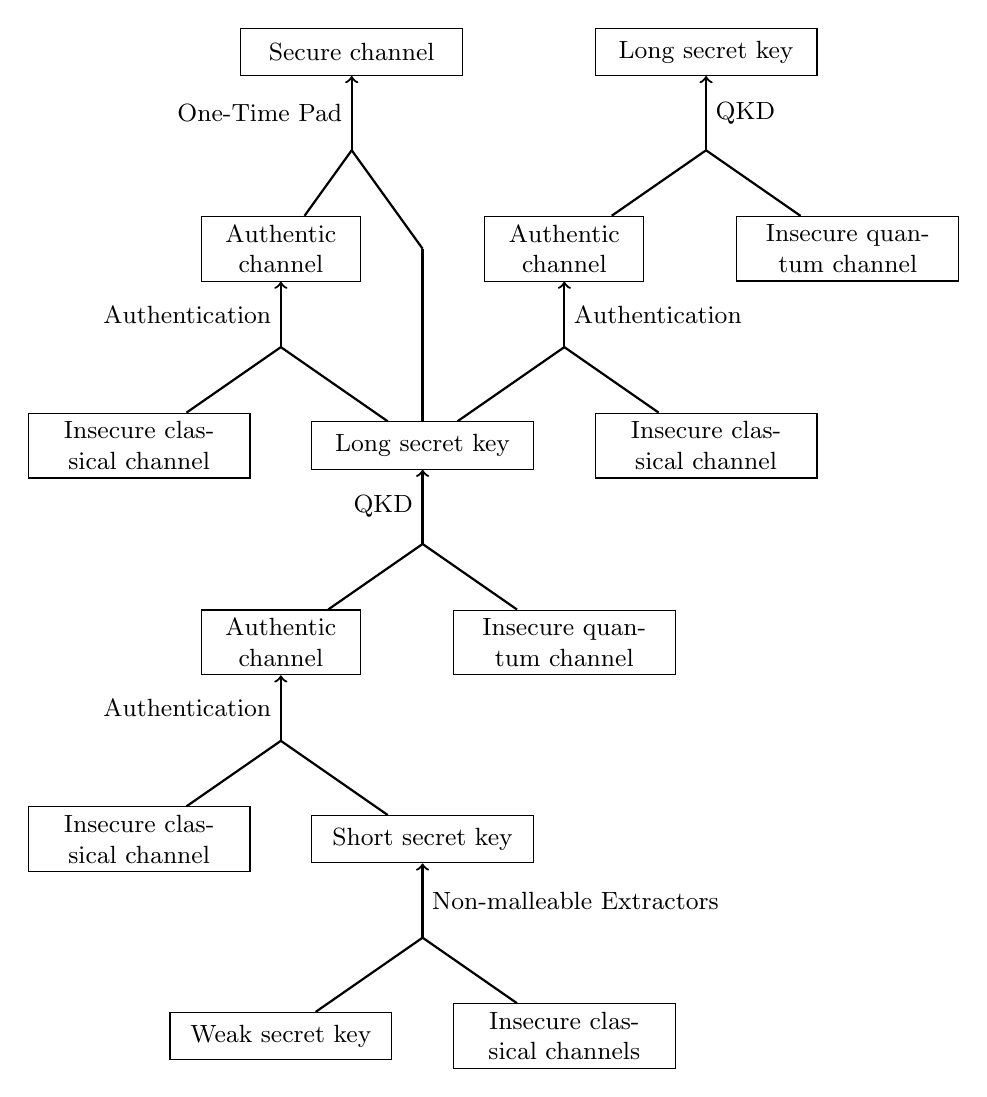
\begin{tikzpicture}[sArrow/.style={-{To[]},thick},
textbox/.style={draw,text width=2.6cm,text centered,minimum height=.6cm}]
\small

\def\d{1.8}
\def\e{2.5}

\node[textbox] (z2) at (1*\d,-1*\e) {Weak secret key};
\node[textbox] (z4) at (3*\d,-1*\e) {Insecure classical channels};
\node[textbox] (a1) at (0*\d,0*\e) {Insecure classical channel};
\node[textbox] (a3) at (2*\d,0*\e) {Short secret key};
\node (m3) at (2*\d,-.5*\e) {};
\node[draw,text width=1.8cm,text centered] (b2) at (1*\d,1*\e) {Authentic channel};
\node (n2) at (1*\d,.5*\e) {};
\node[textbox] (b4) at (3*\d,1*\e) {Insecure quantum channel};
\node[textbox] (c3) at (2*\d,2*\e) {Long secret key};
\node (o3) at (2*\d,1.5*\e) {};
\node[textbox] (c1) at (0*\d,2*\e) {Insecure classical channel};
\node[textbox] (c5) at (4*\d,2*\e) {Insecure classical channel};
\node[draw,text width=1.8cm,text centered] (d2) at (1*\d,3*\e) {Authentic channel};
\node[draw,text width=1.8cm,text centered] (d4) at (3*\d,3*\e) {Authentic channel};
\node (p2) at (1*\d,2.5*\e) {};
\node (p4) at (3*\d,2.5*\e) {};
\node[textbox] (e25) at (1.5*\d,4*\e) {Secure channel};
\node (q3) at (2*\d,3*\e) {};
\node (r25) at (1.5*\d,3.5*\e) {};
\node[textbox] (d6) at (5*\d,3*\e) {Insecure quantum channel};
\node[textbox] (e5) at (4*\d,4*\e) {Long secret key};
\node (r5) at (4*\d,3.5*\e) {};

\draw[thick] (z2) to (m3.center);
\draw[thick] (z4) to (m3.center);
\draw[sArrow] (m3.center) to node[auto,swap] {Non-malleable Extractors} (a3);
\draw[thick] (a1) to (n2.center);
\draw[thick] (a3) to (n2.center);
\draw[sArrow] (n2.center) to node[auto] {Authentication} (b2);
\draw[thick] (b2) to (o3.center);
\draw[thick] (b4) to (o3.center);
\draw[sArrow] (o3.center) to node[auto] {QKD} (c3);
\draw[thick] (c1) to (p2.center);
\draw[thick] (c3) to (p2.center);
\draw[sArrow] (p2.center) to node[auto] {Authentication} (d2);
\draw[thick] (c3) to (p4.center);
\draw[thick] (c5) to (p4.center);
\draw[sArrow] (p4.center) to node[auto,swap] {Authentication} (d4);
\draw[thick] (c3) to (q3.center);
\draw[thick] (d2) to (r25.center);
\draw[thick] (q3.center) to (r25.center);
\draw[sArrow] (r25.center) to node[auto] {One-Time Pad} (e25);
\draw[thick] (d4) to (r5.center);
\draw[thick] (d6) to (r5.center);
\draw[sArrow] (r5.center) to node[auto,swap] {QKD} (e5);

\end{tikzpicture}

\caption[Recursive construction of
resources]{\label{fig:construction}A constructive view of
  cryptography. A cryptographic protocol uses (weak) resources to
  construct other (stronger) resources. These resources are depicted
  in the boxes, and the arrows are protocols. Each box is a
  one-time-use resource, so the same resource appears in multiple
  boxes if different protocols require it. The long secret key
  resource in the center of the figure is split in three shorter keys,
  each of which is used by a separate protocol. The example of secure
  message transmission illustrated here is discussed in detail in
  \secref{sec:smt}.}
\end{figure*}

The resources used and constructed in cryptography are interactive
systems shared between players. A system that distributes secret key
or the different types of channels mentioned in the paragraph above
are examples of such resources. These are formalized on an abstract
level in \secref{sec:ac.systems}, and possible instantiations are
discussed in \secref{sec:ac.instantiating}. Static resources such as
coherent states \cite{BCP14,MZYM19} can be seen as a special case of
these.




\subsection{Example: the one-time pad}
\label{sec:ac.otp}

In this section, we describe how the notions introduced above are
employed to specify the security of a cryptographic protocol. For this
we consider a concrete example, One-Time Pad (OTP)
encryption~\cite{Vernam26}. The OTP assumes that the players have access
to an authentic channel, i.e., one which provides the receiver with
the guarantee that the messages received come from the correct sender,
but there is no guarantee about the secrecy of the messages sent on
such a channel, i.e., they may leak to Eve. The OTP also requires the
players to have access to a secret key. These two resources are drawn
as boxes with square corners in \figref{fig:otp.real}. According to
the protocol, the sender, Alice, encrypts a message~$x$ as
$y \coloneqq x \xor k$, where $k$ is the secret key, and where $\xor$
denotes the bit-wise exclusive OR operation. The ciphertext $y$ is
then sent over an authentic channel to the receiver, Bob, who decrypts
it by carrying out the operation $x = y \xor k$. At the same time, $y$
may also leak to an adversary, Eve.

\begin{figure}[tb]
  \centering
  \subfloat[Real OTP system][\label{fig:otp.real}The real OTP
    system consists of the OTP protocol $(\pi^{\otp}_A,\pi^{\otp}_B)$ together
   a secret key and authentic channel resources.]{
\begin{tikzpicture}[
sArrow/.style={->,>=stealth,thick},
thinResource/.style={draw,thick,minimum width=2cm,minimum height=1cm},
protocol/.style={draw,rounded corners,thick,minimum width=1.3cm,minimum height=2.5cm},
pnode/.style={minimum width=.9cm,minimum height=.5cm}]

\small

\def\t{3.7} %1+1.3+.4+2/1
\def\u{2.05} %1.3/2+.4+2/1
\def\v{.75}

\node[pnode] (a1) at (-\u,\v) {};
\node[pnode] (a2) at (-\u,0) {};
\node[pnode] (a3) at (-\u,-\v) {};
\node[protocol,text width=1.1cm] (a) at (-\u,0) {\footnotesize $y
  =$\\$\quad x \xor k$};
\node[yshift=-2,above right] at (a.north west) {\footnotesize
  $\pi^{\otp}_A$};
\node (alice) at (-\t,0) {Alice};

\node[pnode] (b1) at (\u,\v) {};
\node[pnode] (b2) at (\u,0) {};
\node[pnode] (b3) at (\u,-\v) {};
\node[protocol,text width=1.1cm] (b) at (\u,0) {\footnotesize $x
  =$\\$\quad y \xor k$};
\node[yshift=-2,above right] (blabel) at (b.north west) {\footnotesize $\pi^{\otp}_B$};
\node (bob) at (\t,0) {Bob};

\node[thinResource] (keyBox) at (0,\v) {};
\node[draw] (key) at (0,\v) {key};
\node[yshift=-2,above right] at (keyBox.north west) {\footnotesize Secret key};
\node[thinResource] (channel) at (0,-\v) {};
\node[yshift=-1.5,above right] at (channel.north west) {\footnotesize
  Authentic ch.};
\node (eve) at (0,-2.15) {Eve};
\node (junc) at (eve |- a3) {};

\draw[sArrow] (key) to node[auto,swap,pos=.3] {$k$} (a1);
\draw[sArrow] (key) to node[auto,pos=.3] {$k$} (b1);

\draw[sArrow] (alice) to node[auto,pos=.1] {$x$} (a2);
\draw[sArrow] (b2) to node[auto,pos=.8] {$x$} (bob);

\draw[sArrow] (a3) to node[pos=.13,auto] {$y$} node[pos=.87,auto] {$y$} (b3);
\draw[sArrow] (junc.center) to node[pos=.75,auto] {$y$} (eve);

\node[draw, gray, thick, fit=(a)(b)(blabel), inner sep=6] {};

\end{tikzpicture}}

\vspace{6pt}

\subfloat[Ideal One-Time OTP system][\label{fig:otp.ideal}The ideal
OTP system consists of the ideal secure channel and a simulator
$\sigma^{\otp}_E$.]{
\begin{tikzpicture}[
sArrow/.style={->,>=stealth,thick},
thinResource/.style={draw,thick,minimum width=1.618*2cm,minimum height=1cm},
protocolLong/.style={draw,rounded corners,thick,minimum height=1cm,minimum width=2.8cm}]

\small

\def\t{2.368} % 1.618+.75
\def\u{-.75}
\def\v{.75}
\def\w{-1.75} % .25+1+.5

\node[thinResource] (channel) at (0,\v) {};
\node[yshift=-1.5,above right] (chlabel)at (channel.north west) {\footnotesize
  Secure channel};
\node (alice) at (-2.6,\v) {Alice};
\node (bob) at (2.6,\v) {Bob};

\node[protocolLong] (sim) at (0,\u) {};
\node[xshift=-1.5,yshift=-2,above right] at (sim.north west) {$\sigma^{\otp}_E$};
\node[draw] (rand) at (0,\u) {\footnotesize Random string};


\draw[sArrow] (alice) to node[pos=.03,auto] {$x$}
node[pos=.96,auto] {$x$} (bob);
\draw[sArrow,dotted] (0,\v) to node[pos=.6,auto] {$|x|$} (rand);

\node (eve) at (0,\w-.4) {Eve};
\draw[sArrow] (rand) to node[pos=.75,auto] {$y$} (eve);

\node[draw, gray, thick, fit=(channel)(chlabel)(sim), inner sep=6] {};

\end{tikzpicture}}


\caption[Real and Ideal One-Time Pad systems]{\label{fig:otp}The real
  and ideal one-time pad systems. Boxes with rounded corners are local
  systems executed at Alice's, Bob's or Eve's interfaces. The
  rectangular boxes are shared resources modeling channels or shared
  keys. Arrows represent the
  transmission of messages between systems or to the environment (distinguisher).

  The real world is depicted in
  \subref{fig:otp.real}. The
   protocol consists of a part $\pi^{\otp}_A$ executed by Alice (who
   has access to the interfaces on the left hand side) and a part
    $\pi^{\otp}_B$ executed by Bob (on the right hand side). It
    takes a message $x$ at Alice's outer interface as
    well as a key~$k$, and output a ciphertext $y$ towards the
    authentic channel.  Bob's part of the protocol takes $y$ and~$k$ as
    input, and outputs the decrypted message. The channel may leak~$y$
    at Eve's interface (at the bottom).

    The ideal world is depicted in \subref{fig:otp.ideal}. The secure
    channel transmits the message perfectly from Alice's to Bob's
    interface, leaking only the message length at Eve's interface. The
    simulator $\sigma^{\otp}_E$ generates a random string $y$ of
    length $|x|$, making the real and ideal systems perfectly  indistinguishable.}
\end{figure}

For this example, the goal of the OTP is to add confidentiality to an
authentic channel,\footnote{Alternatively, one may use the OTP with a
  completely insecure channel, and thus obtain a malleable
  confidential channel~\cite{MRT12}.} i.e., the ideal system is a secure
channel, drawn as a box with square corners in
\figref{fig:otp.ideal}. This is a channel which only leaks the message size
but no other information to Eve. It is straightforward to verify that
in the real system, provided that the key~$k$ is uniformly distributed
over bitstrings of the same length as the message~$x$, the ciphertext
$y$ is statistically independent of the message~$x$. The
ciphertext~$y$ hence does not provide Eve with any information
about~$x$, except potentially for its length~$|x|$.  It thus
constructs a secure channel from Alice to Bob. 

% \begin{figure}[tb]


% \begin{tikzpicture}[
% sArrow/.style={->,>=stealth,thick},
% largeResource/.style={draw,thick,minimum width=1.618*2cm,minimum height=2cm}]

% \small

% \node[largeResource] (keyBox) at (0,0) {};
% \node (alice) at (-2.6,0) {Alice};
% \node (bob) at (2.6,0) {Bob};
% \node (eve) at (0,-1.7) {Eve};
% \node (ajunc) at (eve.north |- alice) {};

% \draw[sArrow] (alice) to node[pos=.06,auto] {$x$} node[pos=.94,auto] {$x$} (bob);
% \draw[dotted,sArrow] (ajunc.center) to node[pos=.85,auto,swap] {$|x|$} (eve);

% \end{tikzpicture}


% \caption[Secure channel]{\label{fig:otp.ideal.resource}A secure
%   channel from Alice to Bob leaks only the message size at Eve's interface.}
% \end{figure}

To make the real and ideal systems comparable, we consider an entire class of
systems, which are obtained by appending an arbitrary system, called a
\emph{simulator}, to the Eve interface of the ideal channel
resource. The systems from this class are sometimes called
\emph{relaxations} (of the ideal system). The idea is that none of
these relaxations can be more useful to Eve than the original ideal
channel, because she may always herself carry out the task of the
simulator. Security now means that the real system is
indistinguishable from at least one relaxation of the ideal system. In
our example of the OTP, such a relaxation may be obtained by a
simulator that simply generates a random string of length~$|x|$ and
outputs it at the Eve interface, as depicted in
\figref{fig:otp.ideal}.

To establish security of OTP encryption, it is therefore sufficient to
show that the real system depicted by \figref{fig:otp.real} is
indistinguishable from the relaxation of the ideal secure channel shown in~\figref{fig:otp.ideal}. That is, the two systems must behave
identically when they interact with a distinguisher.  This is indeed
the case. For both of them, if the distinguisher inputs $x$ at Alice's
interface, the same string $x$ is output at Bob's interface and a
uniformly random string of length $|x|$ is output at Eve's
interface. The two systems are thus perfectly indistinguishable \---
if the distinguisher were to take a guess for which of the two it is interacting with, it would be right with
probability exactly $1/2$. In this sense, the OTP construction is
perfectly secure.

If two systems are indistinguishable, they can be used interchangeably in any setting. For example, let some protocol $\pi'$ be proven secure if Alice and Bob are connected by a secure channel. Since the OTP constructs such a channel, it can be used in lieu of the secure channel, and composed with $\pi'$. Or equivalently, the contrapositive: if composing the OTP and $\pi'$ were to leak some vital information, which would not happen with a secure channel, a distinguisher that is either given the real or ideal system could run $\pi'$ internally and check whether this leak occurs to find out with which of the two it is interacting.


% The adversary, Eve, has
% access to her interface only, where the ciphertext $y$ is
% leaked. The distinguisher has access to all interfaces; it can thus
% simulate any setting in which the protocol might be used, in an
% attempt to decide if it is interacting with the real or ideal
% system. Hence, if the real and ideal systems cannot be
% distinguished,

% A simulator connected to the adversary's interface can only weaken
% this player's power: any action performed when connected to the
% simulator's interface could be performed if connected to the ideal
% resource's interface, by

% This simulator can be seen as a
% thought experiment: if such a simulator exists, then a dishonest party
% might as well run the simulator and generate a transcript herself
% instead of attacking the protocol, since this leaks the same
% information and results in the same outcome \--- even from the point
% of view of the global distinguisher.


% \subsubsection{Metric}
% \label{sec:ac.overview.metric}


\subsection{Abstract theory of cryptographic systems}
\label{sec:ac.systems}

The previous sections introduced the concepts of resources, protocols
and simulators in an informal manner. Now, following the spirit of the
AC framework described in \secref{sec:ac.ac}), we provide an axiomatic specification of these
concepts. This will allow us to give a definition of cryptographic security, which is precise, but at the same time largely independent of
implementation details. In particular, it does not depend on the underlying computational model or the scheduling of messages exchanged between the systems. 

While this abstract approach to defining security is rather universal, we note that, when describing concrete systems and
their compositions such as those 
depicted in \figref{fig:otp}, their behaviour must of course be
specified in detail. This may be done using various
frameworks for modeling interactive (quantum) systems, e.g., the
Quantum Combs of \textcite{CDP09} or the Causal Boxes of
\textcite{PMMRT17}. This is discussed further in
\secref{sec:ac.instantiating}.

Nevertheless, the definitions that now follow refer to an abstract notion of a \emph{system}. Following the idea of abstraction motivated above, and  continuing the analogy to group theory used in \secref{sec:ac.ac}, it is sufficient to think of systems as objects on which certain operations are defined, such as their composition.  We will consider two types of systems, which we call resources and converters, and which have slightly different properties.

\paragraph{Resources.} A \emph{resource} is a system with
interfaces specified by a set $\cI$ (e.g., $\cI = \{A,B,E\}$).  
Each
interface $i \in \cI$ models how a player~$i$ can access the system
(e.g., provide inputs and read outputs). Examples of resources are a communication channel or any of the objects that appears in Fig.~\ref{fig:construction} as a box. We will sometimes use the term \emph{$\cI$-resource} to specify the interface set. Resources are equipped with
a parallel composition operator, denoted by~$\|$, that maps two $\cI$-resources to
another $\cI$-resource.

\paragraph{Converters.} A \emph{converter} is a system with two
interfaces, an \emph{inside} interface and an \emph{outside}
interface. A converter can be appended to a resource, converting it
into a new resource. For this the inside interface connects to an
interface of a resource, and the outside interface becomes the new
interface of the new resource \--- see the OTP example in
\figref{fig:otp}, where the gray boxes are new resources resulting
from composing resources and converters. We write either
$\alpha_i \aR$ or $\aR\alpha_i$ to denote the new resource with the
converter $\alpha$ connected at the interface $i$ of
$\aR$.\footnote{There is no mathematical difference between
  $\alpha_i \aR$ and $\aR\alpha_i$. It sometimes simplifies the
  notation to have the converters for some players written on the
  right of the resource and the ones for others on the left, rather
  than having all of them at the same side, hence the two notations.}
Simulators and protocols are examples of converters (see below).

Converters can be composed among themselves. There are two ways of
doing this, referred to as serial and parallel composition. These are
defined as
\begin{align*} %\label{eq:axioms.order}
(\alpha\beta)_i \aR & \coloneqq
  \alpha_i (\beta_i \aR) \\ \intertext{and}  (\alpha \| \beta)_i
  (\aR\|\aS) & \coloneqq (\alpha_i \aR) \| (\beta_i \aS), \end{align*}
  respectively. 
  
  \paragraph{Protocols.} A \emph{(cryptographic) protocol} is a family
  $\alpha = \{\alpha_i\}_i$, of converters (one for every honest
  player). A protocol can be applied to a resource $\aR$, giving a new
  resource denoted by $\alpha\aR$ or $\aR\alpha$. This resource is
  obtained by connecting each member of the family to the interface
  specified by its index.

  % \paragraph{Filters and filtered resources.} A \emph{filter} is a
  % specific converter that, when applied to an interface of a resource,
  % ``blocks'' that interface, i.e., it prevents any outside access to
  % the interface. Filters are often denoted by $\sharp$ or
  % $\lozenge$. A \emph{filtered resource}, denoted by $\aR_\sharp$, is
  % a pair consisting of a resource $\aR$ and a filter $\sharp$. Filters
  % are used to describe the behaviour of a potentially adversarial
  % interface of a resource when no adversary is present. That is, a
  % resource $\aR$ is supposed to behave like $\aR\sharp_E$ in the
  % absence of an adversary.

  \paragraph{Metric.} As explained in \secref{sec:ac.realideal}, the
  distance between resources can be quantified using the notion of
  distinguishers. More generally, one may in principle
  consider any arbitrary pseudo\-/metric, $d(\cdot,\cdot)$, so that
  the following conditions hold:\footnote{If also
    $d(\aR,\aS) = 0 \implies \aR=\aS$ holds then $d$ is a metric.}
\begin{align*} \text{(identity)} & &
  d\left(\aR,\aR\right) & = 0, \\ %\label{eq:pm.ref} \\
  \text{(symmetry)} & & d\left(\aR,\aS\right) & =
  d\left(\aS,\aR\right), \\ %\label{eq:pm.sym} \\
  \text{(triangle inequality)} & & d\left(\aR,\aS\right)
  & \leq d\left(\aR,\aT\right) +
  d\left(\aT,\aS\right). % \label{eq:pm.tri}
\end{align*} Furthermore, the pseudo\-/metric must be non-increasing
under composition with resources and converters.\footnote{This only
  holds for information\-/theoretic security, which is the topic of
  most of this review.} This means that for any converter $\alpha$ and
resources $\aR,\aS,\aT$,
\begin{equation*} %\label{eq:axioms.nonincrease}
d(\alpha\aR,\alpha\aS)
  \leq d(\aR,\aS) \quad \text{and} \quad d(\aR\|\aT,\aS\|\aT) \leq
  d(\aR,\aS). \end{equation*}
In this work we often simply write $\aR \close{\eps} \aS$ instead of
$d(\aR,\aS) \leq \eps$.

%\vspace{\baselineskip}

\subsection{Security definition}
\label{sec:ac.security}

We are now ready to define the security of a cryptographic
protocol. We do so in \defref{def:security} in the three-player
setting, for honest Alice and Bob, and dishonest Eve \--- and
illustrate this definition in Fig.~\ref{fig:security}. Thus, in the
following, all resources have three interfaces, denoted $A$, $B$ and
$E$, and we consider honest behaviors (given by a protocol
$(\pi_A,\pi_B)$) at the $A$- and $B$\=/interfaces, but arbitrary
behavior at the $E$\=/interface. We refer to \textcite{MR11} for the
general case, when arbitrary players can be dishonest.

\begin{figure*}[tb]
% \begin{subfigure}[b]{\textwidth}


% \begin{tikzpicture}[scale=.8,
% sArrow/.style={->,>=stealth,thick},
% largeResource/.style={draw,thick,minimum width=1.618*2cm,minimum height=2cm},
% lrnode/.style={minimum width=1.36*2cm,minimum height=.2cm},
% llrnode/.style={minimum width=.2cm,minimum height=1.5cm},
% tlrnode/.style={minimum width=.2cm,minimum height=.5cm},
% thinResource/.style={draw,thick,minimum width=1.618*2cm,minimum height=1cm},
% filter/.style={draw,thick,minimum width=1.618cm,minimum height=1cm},
% protocol/.style={draw,thick,minimum width=1.545cm,minimum height=2.5cm},
% pnode/.style={minimum width=1cm,minimum height=.5cm}]

% \small

% \def\t{4.422} %.75+1.545+.5+1.618
% \def\u{2.9} %1.545/2+.5+1.618
% \def\v{.6}
% \def\w{1.8}

% \def\a{5.2}
% \def\b{8.3}
% \def\tb{2.368} %.75+1.618
% \def\vb{.4}
% \def\ub{.75}
% \def\wb{2.05}

% \node[scale=.8,pnode] (a1) at (-\u,\v) {};
% \node[scale=.8,pnode] (a2) at (-\u,0) {};
% \node[scale=.8,pnode] (a3) at (-\u,-\v) {};
% \node[scale=.8,protocol] (a) at (-\u,0) {};
% \node[yshift=-2,above right] at (a.north west) {\footnotesize
%   $\pi_A$};
% \node (alice1) at (-\t,\v) {};
% \node (alice2) at (-\t,0) {};
% \node (alice3) at (-\t,-\v) {};

% \node[scale=.8,pnode] (b1) at (\u,\v) {};
% \node[scale=.8,pnode] (b2) at (\u,0) {};
% \node[scale=.8,pnode] (b3) at (\u,-\v) {};
% \node[scale=.8,protocol] (b) at (\u,0) {};
% \node[yshift=-2,above right] at (b.north west) {\footnotesize $\pi_B$};
% \node (bob1) at (\t,\v) {};
% \node (bob2) at (\t,0) {};
% \node (bob3) at (\t,-\v) {};

% \node[scale=.8,lrnode] (r1) at (0,\v) {};
% \node[scale=.8,lrnode] (r2) at (0,0) {};
% \node[scale=.8,lrnode] (r3) at (0,-\v) {};
% \node[scale=.8,llrnode] (rr1) at (-\v,0) {};
% \node[scale=.8,llrnode] (rr2) at (0,0) {};
% \node[scale=.8,llrnode] (rr3) at (\v,0) {};
% \node[scale=.8,largeResource] (R) at (0,0) {};
% \node[yshift=-2,above right] at (R.north west) {\footnotesize $\aR$};

% \node (eve1) at (-\v,-\w) {};
% \node (eve2) at (0,-\w) {};
% \node (eve3) at (\v,-\w) {};

% \node[scale=.8,filter] (fi) at (0,-1.9) {};
% \node[xshift=2,below left] at (fi.north west) {\footnotesize
%   $\sharp_E$};

% \draw[sArrow] (alice1) to (a1);
% \draw[sArrow] (a2) to (alice2);
% \draw[sArrow] (alice3) to (a3);

% \draw[sArrow] (a1) to (r1);
% \draw[sArrow] (r2) to (a2);
% \draw[sArrow] (a3) to (r3);

% \draw[sArrow] (r1) to (b1);
% \draw[sArrow] (b2) to (r2);
% \draw[sArrow] (r3) to (b3);

% \draw[sArrow] (b1) to (bob1);
% \draw[sArrow] (bob2) to (b2);
% \draw[sArrow] (b3) to (bob3);

% \draw[sArrow] (rr1) to (eve1);
% \draw[sArrow] (eve2) to (rr2);
% \draw[sArrow] (rr3) to (eve3);

% \node at (\a,0) {\Large $\close{\eps}$};

% \node[scale=.8,lrnode] (s1) at (\b,\vb+\ub) {};
% \node[scale=.8,lrnode] (s2) at (\b,\ub) {};
% \node[scale=.8,lrnode] (s3) at (\b,-\vb+\ub) {};
% \node[scale=.8,tlrnode] (ss1) at (\b-\v,\ub) {};
% \node[scale=.8,tlrnode] (ss2) at (\b,\ub) {};
% \node[scale=.8,tlrnode] (ss3) at (\b+\v,\ub) {};
% \node[scale=.8,thinResource] (S) at (\b,\ub) {};
% \node[yshift=-2,above right] at (S.north west) {\footnotesize $\aS$};

% \node[scale=.8,tlrnode] (t1) at (\b-\v,-\ub) {};
% \node[scale=.8,tlrnode] (t2) at (\b,-\ub) {};
% \node[scale=.8,tlrnode] (t3) at (\b+\v,-\ub) {};
% \node[scale=.8,filter] (fil) at (\b,-\ub) {};
% \node[xshift=-2,below right] at (fil.north east) {\footnotesize $\lozenge_E$};

% \node (cate1) at (\b-\tb,\vb+\ub) {};
% \node (cate2) at (\b-\tb,\ub) {};
% \node (cate3) at (\b-\tb,-\vb+\ub) {};

% \node (dave1) at (\b+\tb,\vb+\ub) {};
% \node (dave2) at (\b+\tb,\ub) {};
% \node (dave3) at (\b+\tb,-\vb+\ub) {};

% \draw[sArrow] (cate1) to (s1);
% \draw[sArrow] (s2) to (cate2);
% \draw[sArrow] (cate3) to (s3);

% \draw[sArrow] (s1) to (dave1);
% \draw[sArrow] (dave2) to (s2);
% \draw[sArrow] (s3) to (dave3);

% \draw[sArrow] (ss1) to (t1);
% \draw[sArrow] (t2) to (ss2);
% \draw[sArrow] (ss3) to (t3);

% \end{tikzpicture}


% \caption[Completeness]{\label{fig:security.availability}Condition
%   \eqref{eq:def.cor} from \defref{def:security}. If Eve's interfaces
%   are blocked by filters emulating honest behavior, the functionality
%   constructed by the protocol should be indistinguishable from the
%   ideal resource.}
% \end{subfigure}

% \vspace{12pt}

% \begin{subfigure}[b]{\textwidth}


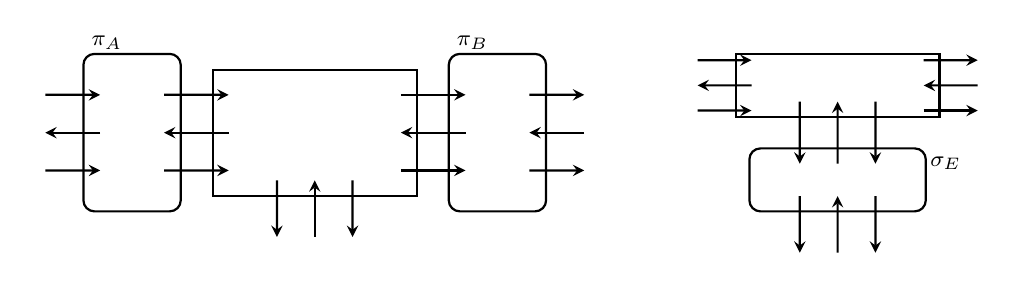
\begin{tikzpicture}[scale=.8,
sArrow/.style={->,>=stealth,thick},
largeResource/.style={draw,thick,minimum width=1.618*2cm,minimum height=2cm},
lrnode/.style={minimum width=1.36*2cm,minimum height=.2cm},
llrnode/.style={minimum width=.2cm,minimum height=1.5cm},
tlrnode/.style={minimum width=.2cm,minimum height=.5cm},
thinResource/.style={draw,thick,minimum width=1.618*2cm,minimum height=1cm},
%filter/.style={draw,thick,minimum width=1.618cm,minimum height=1cm},
protocol/.style={draw,rounded corners,thick,minimum width=1.545cm,minimum height=2.5cm},
pnode/.style={minimum width=1cm,minimum height=.5cm},
protocolLong/.style={draw,rounded corners,thick,minimum height=1cm,minimum width=2.8cm}]


\small

\def\t{4.422} %.75+1.545+.5+1.618
\def\u{2.9} %1.545/2+.5+1.618
\def\v{.6}
\def\w{1.8}

\def\a{5.2}
\def\b{8.3}
\def\tb{2.368} %.75+1.618
\def\vb{.4}
\def\ub{.75}
\def\wb{2.05}

\node[scale=.8,pnode] (a1) at (-\u,\v) {};
\node[scale=.8,pnode] (a2) at (-\u,0) {};
\node[scale=.8,pnode] (a3) at (-\u,-\v) {};
\node[scale=.8,protocol] (a) at (-\u,0) {};
\node[yshift=-2,above right] at (a.north west) {\footnotesize
  $\pi_A$};
\node (alice1) at (-\t,\v) {};
\node (alice2) at (-\t,0) {};
\node (alice3) at (-\t,-\v) {};

\node[scale=.8,pnode] (b1) at (\u,\v) {};
\node[scale=.8,pnode] (b2) at (\u,0) {};
\node[scale=.8,pnode] (b3) at (\u,-\v) {};
\node[scale=.8,protocol] (b) at (\u,0) {};
\node[yshift=-2,above right] at (b.north west) {\footnotesize $\pi_B$};
\node (bob1) at (\t,\v) {};
\node (bob2) at (\t,0) {};
\node (bob3) at (\t,-\v) {};

\node[scale=.8,lrnode] (r1) at (0,\v) {};
\node[scale=.8,lrnode] (r2) at (0,0) {};
\node[scale=.8,lrnode] (r3) at (0,-\v) {};
\node[scale=.8,llrnode] (rr1) at (-\v,0) {};
\node[scale=.8,llrnode] (rr2) at (0,0) {};
\node[scale=.8,llrnode] (rr3) at (\v,0) {};
\node[scale=.8,largeResource] (R) at (0,0) {};
\node[yshift=-2,above right] at (R.north west) {\footnotesize $\aR$};

\node (eve1) at (-\v,-\w) {};
\node (eve2) at (0,-\w) {};
\node (eve3) at (\v,-\w) {};

\draw[sArrow] (alice1) to (a1);
\draw[sArrow] (a2) to (alice2);
\draw[sArrow] (alice3) to (a3);

\draw[sArrow] (a1) to (r1);
\draw[sArrow] (r2) to (a2);
\draw[sArrow] (a3) to (r3);

\draw[sArrow] (r1) to (b1);
\draw[sArrow] (b2) to (r2);
\draw[sArrow] (r3) to (b3);

\draw[sArrow] (b1) to (bob1);
\draw[sArrow] (bob2) to (b2);
\draw[sArrow] (b3) to (bob3);

\draw[sArrow] (rr1) to (eve1);
\draw[sArrow] (eve2) to (rr2);
\draw[sArrow] (rr3) to (eve3);

\node at (\a,0) {\Large $\close{\eps}$};

\node[scale=.8,lrnode] (s1) at (\b,\vb+\ub) {};
\node[scale=.8,lrnode] (s2) at (\b,\ub) {};
\node[scale=.8,lrnode] (s3) at (\b,-\vb+\ub) {};
\node[scale=.8,tlrnode] (ss1) at (\b-\v,\ub) {};
\node[scale=.8,tlrnode] (ss2) at (\b,\ub) {};
\node[scale=.8,tlrnode] (ss3) at (\b+\v,\ub) {};
\node[scale=.8,thinResource] (S) at (\b,\ub) {};
\node[yshift=-2,above right] at (S.north west) {\footnotesize $\aS$};

\node[scale=.8,tlrnode] (t1) at (\b-\v,-\ub) {};
\node[scale=.8,tlrnode] (t2) at (\b,-\ub) {};
\node[scale=.8,tlrnode] (t3) at (\b+\v,-\ub) {};
\node[scale=.8,protocolLong] (sim) at (\b,-\ub) {};
\node[xshift=-2,below right] at (sim.north east) {\footnotesize $\sigma_E$};

\node (cate1) at (\b-\tb,\vb+\ub) {};
\node (cate2) at (\b-\tb,\ub) {};
\node (cate3) at (\b-\tb,-\vb+\ub) {};

\node (dave1) at (\b+\tb,\vb+\ub) {};
\node (dave2) at (\b+\tb,\ub) {};
\node (dave3) at (\b+\tb,-\vb+\ub) {};

\node (finn1) at (\b-\v,-\wb) {};
\node (finn2) at (\b,-\wb) {};
\node (finn3) at (\b+\v,-\wb) {};

\draw[sArrow] (cate1) to (s1);
\draw[sArrow] (s2) to (cate2);
\draw[sArrow] (cate3) to (s3);

\draw[sArrow] (s1) to (dave1);
\draw[sArrow] (dave2) to (s2);
\draw[sArrow] (s3) to (dave3);

\draw[sArrow] (ss1) to (t1);
\draw[sArrow] (t2) to (ss2);
\draw[sArrow] (ss3) to (t3);

\draw[sArrow] (t1) to (finn1);
\draw[sArrow] (finn2) to (t2);
\draw[sArrow] (t3) to (finn3);

\end{tikzpicture}


% \caption[Soundness]{\label{fig:security.active}Condition \eqref{eq:def.sec}
%   from \defref{def:security}. If Eve accesses her cheating interface
%   of $\aR$, the resulting system must be simulatable in the ideal
%   world by a converter $\sigma_E$ that only accesses Eve's interface
%   of the ideal resource $\aS$.}
% \end{subfigure}

\caption[Cryptographic security]{\label{fig:security}A depiction of
  \defref{def:security}: a protocol $(\pi_A,\pi_B)$ constructs
  $\aS$ from $\aR$ within $\eps$ if the condition
  illustrated in this figure holds. The sequences of arrows at the
  interfaces between the objects represent (arbitrary) rounds of
  communication.}
\end{figure*}

\begin{deff}[Cryptographic security~\cite{MR11}] \label{def:security}
  Let $\pi_{AB} = (\pi_A,\pi_B)$ be a protocol and $\aR$ and $\aS$ two
   resources.  We say that \emph{$\pi_{AB}$ constructs $\aS$
    from $\aR$ within $\eps$}, denoted by
  \[ 
    \aR \xrightarrow{\pi,\eps} \aS \ ,
  \]
  if there exists a converter $\sigma_E$ (called \emph{simulator})
  such that
   \begin{equation} \label{eq:def.sec} d(\pi_{AB}\aR,\aS\sigma_E) \leq
     \eps.\end{equation} If it is clear from the context what
   resources $\aR$ and $\aS$ are meant, we simply say that $\pi_{AB}$
   is $\eps$\=/secure.
\end{deff}

Although this security definition does not refer to any computational
notions, one usually only considers protocols whose converters are
computationally efficient.\footnote{In principle, any reasonable
  notion of efficiency could be considered here. However, if one takes
  the common asymptotic notion of computational complexity classes,
  one would need to describe systems in terms of a computational model
  that enables such asymptotic considerations.}  Furthermore, if one
requires security to hold under composition with protocols that have
only computational security, it is necessary to restrict the choice of
the simulator $\sigma_E$ to converters that are computationally
efficient.  All the converters and resources considered in this work
are efficient in the standard sense, so we will not mention this any
further.

For a given protocol, we usually want to make several security
statements, e.g., one about what is achieved in the presence of an
adversary (sometimes referred to as either the \emph{soundness} or
\emph{security} of a protocol), another about what is achieved when no
adversary is present (usually called either \emph{completeness} or
\emph{correctness}\footnote{In the QKD literature, correctness has
  another meaning \--- it captures the property that Alice and Bob end
  up with identical keys when Eve is active. The term
  \emph{robustness} is traditionally used in the QKD literature to
  denote the performance of a QKD protocol under honest (noisy)
  conditions. We refer to \secref{sec:security.rob} for a discussion
  of the relation between completeness and robustness.}). These two
cases are captured by considering different resources $\aR$ and $\aS$,
but the same protocol $\pi_{AB}$. We will illustrate this in
\secref{sec:qkd} for the case of QKD.

% The first condition, (\ref{eq:def.cor}), of
% Definition~\ref{def:security} measures how close the constructed
% resource is to the ideal resource in the case where no malicious
% player is intervening. We refer to this condition as capturing the
% \emph{completeness} of a protocol. The second condition,
% (\ref{eq:def.sec}), captures security in the presence of an adversary,
% which we call the \emph{soundness} of the protocol. These two
% equations are illustrated in \figref{fig:security}.


%\paragraph{Composability.}
If two protocols $\pi$ and $\pi'$ are
$\eps$- and $\eps'$\=/secure, the composition of the two is
$(\eps+\eps')$\=/secure. More precisely, let protocols $\pi$ and
$\pi'$ construct $\aS$ from $\aR$ and $\aT$
from $\aS$ within $\eps$ and $\eps'$, respectively,
i.e.,
\[\aR \xrightarrow{\pi,\eps}\aS \qquad \text{and}
  \qquad \aS \xrightarrow{\pi',\eps'}\aT.\] It is
then a consequence of the triangle inequality of the distinguishing
metric that $\pi'\pi$ constructs $\aT$ from $\aR$
within $\eps+\eps'$,
\[\aR \xrightarrow{\pi'\pi,\eps+\eps'}\aT.\] A similar
statement holds for parallel composition. Let $\pi$ and $\pi'$
construct $\aS$ and $\aS'$ from $\aR$ and
$\aR'$ within $\eps$ and $\eps'$, respectively, i.e.,
\[\aR \xrightarrow{\pi,\eps}\aS \qquad \text{and}
\qquad \aR' \xrightarrow{\pi',\eps'} \aS'.\]
If these resources and protocols are composed in parallel, we find that $\pi \| \pi'$ constructs $\aS \| \aS'$ from $\aR \| \aR'$ within $\eps+\eps'$, 
\[\aR \| \aR' \xrightarrow{\pi \| \pi',\eps+\eps'}
\aS \| \aS'.\]
% where $\aR_\sharp \| \aR'_\flat \coloneqq \left(\aR \| \aR',\sharp \|
%   \flat\right)$
% is the filtered resource consisting of the parallel composition of the resources and filters from $\aR_\sharp$ and $\aR'_\flat$. 
Proofs of these statements can be found in \textcite{MR11,Mau12}.
% We illustrate this with several
% examples in \secref{sec:ex} and \appendixref{app:ex.auth}, and sketch
% a generic proof in \appendixref{app:generic}.


\subsection{Interpretation of the security parameter}
\label{sec:ac.interpretation}

Any pseudo\-/metric which satisfies the basic axioms can be used in
\defref{def:security}. However, the usual pseudo\-/metric is the
\emph{distinguishing advantage}, which was introduced in
\eqnref{eq:adv1} in \secref{sec:ac.realideal}. For two resources $\aR$
and $\aS$ and a distinguisher $\fD$, \eqnref{eq:adv1} may be rewritten
as
  \begin{equation}
  \label{eq:adv2} 
    d^{\fD}\left(\aR,\aS\right) \coloneqq \left| \Pr[\fD(\aR) = 0] - \Pr[\fD(\aS) = 0] \right|,
  \end{equation}
  where $\fD(\aR)$ and $\fD(\aS)$ are the random variables
  corresponding to the output of the distinguisher when interacting
  with $\aR$ and $\aS$, respectively. Alternatively, one may
    define the distinguishing advantage for $\fD$ as
\begin{equation}
  \label{eq:adv3}
  d^{\fD}\left(\aR,\aS\right) \coloneqq \left| 2\ddistinguish{\aR,\aS} - 1
  \right|,
\end{equation}
where $\ddistinguish{\aR,\aS}$ is the probability for $\fD$ to
correctly guess with which of $\aR$ or $\aS$ it is interacting when
either one is chosen with probability $1/2$, i.e.,
\[\ddistinguish{\aR,\aS} \coloneqq \frac{1}{2} \Pr[\fD(\aR) = 0] + \frac{1}{2}
  \Pr[\fD(\aS) = 1].\] It is easy to see that \eqnsref{eq:adv2} and
\eqref{eq:adv3} are equivalent.

One then takes the supremum of this expression over all distinguishers
$\fD$ of a given class $\bD$, i.e.,
  \begin{equation}
  \label{eq:adv4} 
  d^{\bD}\left(\aR,\aS\right)  \coloneqq \sup_{\fD \in \bD} d^{\fD}\left(\aR,\aS\right).
  \end{equation}
  The class $\bD$ may be restricted to a particular set of systems
  (e.g., those that are computationally efficient). The strongest
  security notion corresponds to not imposing any restriction on the
  set of distinguishers (beyond what is allowed by physical laws),
  which is the one considered in most of this work, and which we
  denote
\[
  d(\aR,\aS) \leq \eps \qquad \text{or} \qquad \aR \close{\eps} \aS.
\]
  
The distinguishing advantage is of particular importance because it
has an operational interpretation. If the distinguisher notices a
difference between the two, then something in the real setting did not
behave ideally. This can be loosely interpreted as a failure
occurring. If a distinguisher can guess correctly with probability $1$
with which system it is interacting (i.e.,
$\distinguish{\aR,\aS} = 1$), a failure must occur systematically. If,
conversely, it can only guess correctly with probability $1/2$ (which
corresponds to a random guess), this means that the real system always
behaves like the ideal one, hence no failure occurs at all. The
practically relevant cases are those in between. As shown in
\appendixref{app:op}, a guessing probability
$ \distinguish{\aR,\aS} = p$ corresponds to a failure with probability
$\eps = 2p-1$, which is exactly the distinguishing advantage. The
latter can thus be interpreted as the probability that a failure
occurs in the real protocol. This operational interpretation is
crucial for applications, where one must be able to specify what
maximum value $\eps$ one is ready to tolerate.

A bound on the security $\eps$ of a protocol does however not tell us how ``bad'' this failure is. For example, a key distribution protocol which produces perfectly uniform keys for Alice and Bob, but with probability $\eps$ the keys of Alice and Bob are different, is $\eps$\=/secure. Likewise, a protocol which gives $1$ bit of the key to Eve with probability $\eps$, but is perfect otherwise, and another protocol which gives the entire key to Eve with probability $\eps$, but is perfect otherwise, are both $\eps$\=/secure as well. One could argue that leaking the entire key is worse than leaking one bit, which is worse than not leaking anything but generating mismatching keys, and this should be reflected in the level of security of the protocol. However, leaking one bit can be as bad as leaking the entire key if only one bit of the message is vital, and this happens to be the bit obtained by Eve. Having mismatching keys and therefore misinterpreting a message could have more dire consequences than leaking the message to Eve. How bad a failure is depends on the use of the protocol, and since the purpose of cryptographic security is to make a security statement that is valid for all contexts, bounding the probability that a failure (grave or not) occurs, is the best it can do.

The above is particularly relevant if one considers larger cryptographic tasks that may, for instance, use key distribution numerous times as a subprotocol. Since, as described, a security bound gives no idea of the gravity of a failure, the failure of the key distribution protocol could have an impact on the entire cryptographic system. For example, if the key is used to authenticate later communication, the security of the latter may  be affected by a failure in key distribution. This makes it necessary to choose the probability $\eps$ of a failure in any protocol small enough so that the accumulation of all possible failure probabilities used for the larger cryptographic task are still small.  One way of doing this is to increase the security parameter of a protocol on a regular basis, e.g., once a year the parameters are tweaked so that the new probability of a failure is divided by two. If the accumulated failure during the first year is given by $\eps$, then the total failure over an arbitrarily long lifetime of the system is bounded by $2\eps > \eps + \eps/2 + \eps/4 + \dotsc$


\subsection{Instantiating systems}
\label{sec:ac.instantiating}

As mentioned previously, specifying a concrete behavior of a system
requires a model of systems that satisfies the axioms presented in
\secref{sec:ac.systems}, i.e., provides composition and a
pseudo\-/metric with the required properties. In most of this review
we consider interactive quantum systems with sequential scheduling,
i.e., a system receives a (quantum) message, then sends a (quantum)
message, then receives a (quantum) message, etc. Such systems were
analyzed independently by
\textcite{GW07,CDP09,Har11,Gut12,Har12,Har15} [see also
\textcite{Har05,Har07}], to which we refer in the following using the
term from \textcite{CDP09}, namely \emph{quantum combs}. Quantum combs
are a generalization of \emph{random systems}~\cite{Mau02,MPR07} to
quantum information theory.

What these works essentially show is that an interactive system which
receives the $i^{\text{th}}$ input in register $A_i$ and produces the
$i^{\text{th}}$ output in register $B_i$ and which processes $n$
inputs can be fully described by a completely\-/positive, trace
preserving (CPTP) map
\[ \cE : \cL\left(\bigotimes_{i = 1}^n \hilbert_{A_i}\right) \to
  \cL\left(\bigotimes_{i = 1}^n \hilbert_{B_i}\right).\] Conversely,
any such CPTP map corresponds to an interactive system if it respects
causality, i.e., if for any $j \leq n$ and any
$\rho,\sigma \in \cL\left(\bigotimes_{i = 1}^n \hilbert_{A_i}\right)$
with $\trace[A_{>j}]{\rho} = \trace[A_{>j}]{\sigma}$ we have
\[ \ktrace[B_{>j}]{\cE(\rho)} = \ktrace[B_{>j}]{\cE(\sigma)},\] where
$X_{>j} \coloneqq \bigotimes_{i = j+1}^nX_i$.

Systems such as the resources and converters for the one-time pad in
\figref{fig:otp} \--- or the quantum key distribution systems that
will come in \secref{sec:qkd} \--- all correspond to specific quantum
combs. (Nonetheless we usually give informal descriptions of such systems,
rather than using the comb formalism, especially when the details of their behaviour is not relevant for our claims.) The only results discussed in this
work that cannot be modelled as quantum combs are the relativistic
systems reviewed in \secref{sec:relativistic}, which require a more
complex model of systems that can capture space\-/time and also
satisfies the required axioms, e.g., the causal boxes from
\textcite{PMMRT17}.

%%% Local Variables:
%%% TeX-master: "main.tex"
%%% End:
